\documentclass[11pt]{article}
\usepackage{fancyhdr}
\usepackage[vmargin=3.5cm, hmargin=2cm]{geometry}
\usepackage{amsmath, amsfonts, amsthm}
\usepackage{graphicx}
\usepackage{moreverb}
\usepackage{enumerate}
\usepackage{bm}
\usepackage[tiny,compact]{titlesec}
\pagestyle{fancy}
\headheight 14pt
\lhead{UC Berkeley}
\chead{}
\rhead{Stat 88 Fall 2016}
\rfoot{}
\cfoot{\thepage}
\lfoot{}

\parindent0pt  % to stop indenting paragraphs
\parskip1.5ex  % to insert vertical space between paragraphs

% Different font in captions
\newcommand{\captionfonts}{\small}

\makeatletter  % Allow the use of @ in command names
\long\def\@makecaption#1#2{%
  \vskip\abovecaptionskip
  \sbox\@tempboxa{{\captionfonts #1: #2}}%
  \ifdim \wd\@tempboxa >\hsize
    {\captionfonts #1: #2\par}
  \else
    \hbox to\hsize{\hfil\box\@tempboxa\hfil}%
  \fi
  \vskip\belowcaptionskip}
\makeatother   % Cancel the effect of \makeatletter

\newcommand{\V}{\mathrm{Var}}
\newcommand{\E}{\mathbb{E}}
\newcommand{\mbf}{\mathbf}
\newcommand{\mr}{\mathrm}
\newcommand{\yiobs}{Y_i^\mr{obs}}
\newcommand{\yobs}{Y^\mr{obs}}
\newcommand{\yimis}{Y_i^\mr{mis}}
\newcommand{\ymis}{Y^\mr{mis}}
\newcommand{\N}{\mathcal{N}}
\newcommand{\utilde}{\underset{\widetilde{}}}
\newcommand{\txt}{\texttt}

\begin{document}
\centerline{\textbf{Notes on Probability Mass Functions}}
\section*{Probability Mass Functions}
{\bf Note:} I'm not going to refer to the sample space $\Omega$ in the main body of these notes.

In class we talked about random variables $X$, which we think of formally as numerical summaries of a random process.
For example:
\begin{itemize}
\item You roll a die several times and want to summarize this process with $X$, the number of unique faces that we saw.
\item You enter a raffle many times, and want to summarize this process with $X$, the amount of money that you won overall.
\item You record the license plates of cars that drive by your apartment and summarize this process with $X$, the proportion of license plates that come from other states (not California).
\end{itemize}

Just as a random process can give you a different outcome each time you repeat it, the random variable $X$ that summarizes that process can take on different values.
We call the set of values that $X$ can potentially take the \emph{range} or \emph{support} of $X$, and write it as $\mathcal X$. The \emph{distribution} of $X$ defines
how likely $X$ is to take any one of the values in its range $\mathcal X$. For the examples we consider in this class, where the range $\mathcal X$ is finite (that is, $X$ can only take
finitely many values), we can represent this distribution using a \emph{probability mass function}, or pmf for short\footnote{The range of $\mathcal X$ of a random variable $X$ is \emph{not} the same as the sample space $\Omega$. $\Omega$ is the \emph{domain} of $X$; $X$ takes outcomes in the sample space $\Omega$ and summarizes them with a number contained in its range $\mathcal X$. In general, $\Omega$ is a set of full descriptions of ways that the random process could have turned out (e.g., sequences of heads and tails), but $\mathcal X$ is a set of numbers.}.

A probability mass function (pmf) takes any value $k \in \mathcal X$ (that is, any value, which we will write as $k$, from the range $\mathcal X$), and returns the probability that $X$ will take that value. We write this function using the notation $P(X = k)$.

Note that the symbol $k$ here is just a placeholder variable for the \emph{argument} of the pmf. We could equivalently use $x$ or $\heartsuit$ here, and write the same pmf as $P(X = x)$ or $P(X = \heartsuit)$. The important thing is that the pmf is a \emph{function} of the placeholder variable.

\subsection*{Example: Binomial Random Variable}

In class, we talked a binomial random variable $X$ that we define as follows: Flip a coin $n$ times. Each flip of the coin is independent, and has probability $p$ of coming up heads. Define $X$ as the number of heads that we see after flipping the coin $n$ times.

In this case, the range of $X$ is $\mathcal X = \{0, \cdots, n\}$, since we can see as few as $0$ heads or as many as $n$ heads. The probability mass function for $X$ is, for any $k \in \mathcal X$ (or any $\heartsuit \in \mathcal X$):
$$
P(X = k) = {n \choose k} p^k (1-p)^{n-k}\hspace{1em}\textrm{, or equivalently, } \hspace{1em}P(X = \heartsuit) = {n \choose \heartsuit} p^{\heartsuit} (1-p)^{n-\heartsuit}
$$

Using this function, you can answer any question of the form ``What is the probability that we see $m$ heads?'' by plugging in $m$ for $k$ and evaluating the expression. For example, if $n$ is greater than or equal to 10 and we ask, ``What is the probability that we see $10$ heads?'', we can plug in $10$ for $k$ and get our answer:
$$
P(X = 10) = {n \choose 10} p^{10} (1-p)^{n-10}.
$$

\section*{Visualization}
Probability mass functions are useful for visualizing the distributions of random variables. For each value $k \in \mathcal X$, we can plot the probability that $X$ takes this value. Thus, the probability mass function tells you exactly how to draw a distribution plot. It can be intuitive to think that whenever we define a probability mass function, we are actually defining one of these plots.

\subsection*{Example: Binomial Distribution Plots}
Using the pmf defined in the last example, if we supply a number of coin flips $n$ and a probability of flipping heads $p$, we can plot the distribution of $X$, the number of heads that we would see if we flipped this coin $n$ times.

For example, here are the distribution plots for three different settings of $n$ and $p$:

\begin{figure}[h!]
\centering
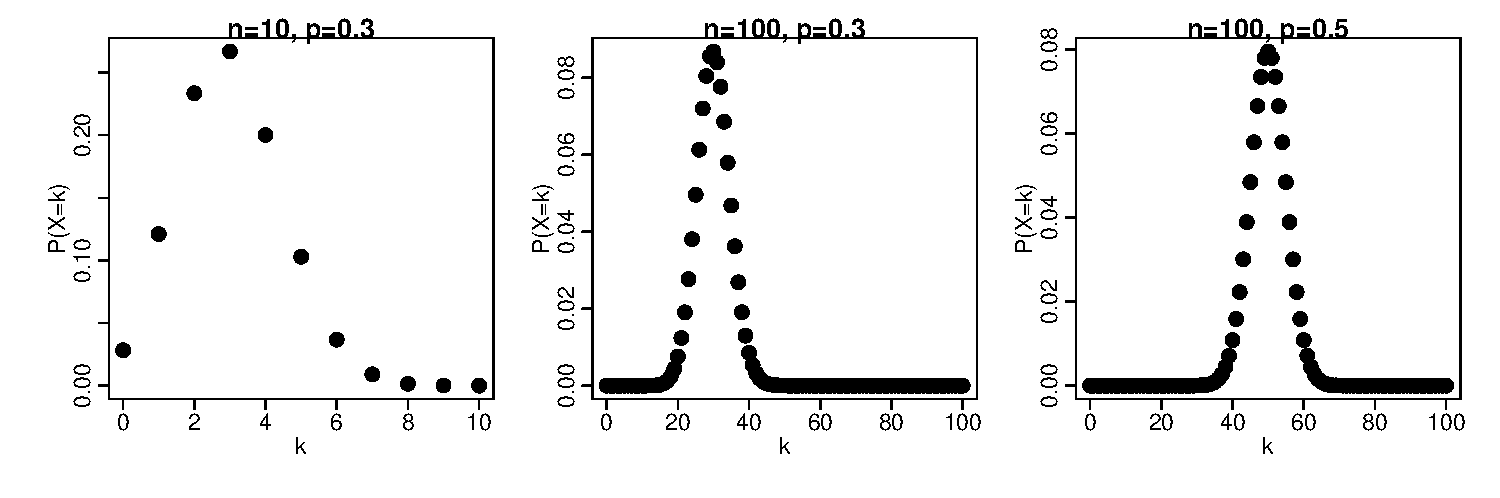
\includegraphics[width=\textwidth]{images/bins.pdf}
\end{figure}

These visualizations help us make observations like the following. When we run a coin flipping procedure like the one described:
\begin{itemize}
\item In all three cases, the most likely value that $X$ (the number of heads) will take is $np$.
\item It is very unlikely that we'll see $X$ take a value in certain parts of the range $\mathcal X$. For example, in both cases where $n = 100$, it's very rare to see a number of heads that differs from the most likely value $np$ by more than 10 heads.
\end{itemize}
\end{document}
